\documentclass[tikz,border=10pt]{standalone}
% Only base TikZ is needed: no extra libraries
\begin{document}
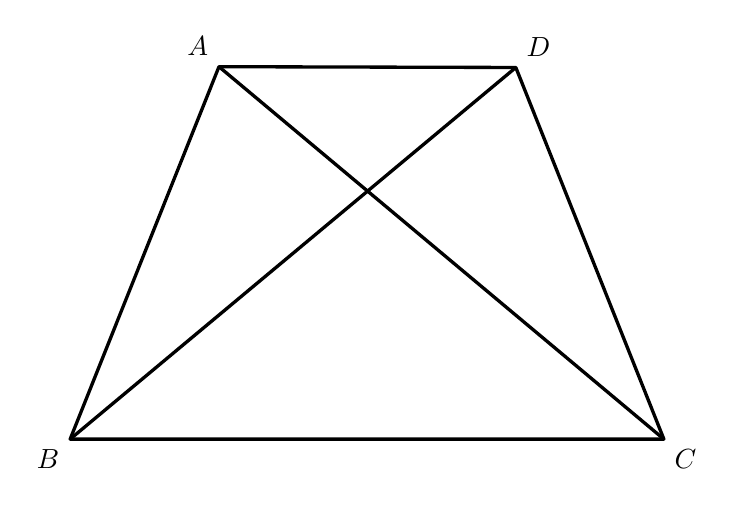
\begin{tikzpicture}[line width=1.2pt, line join=round]
  % Vertices: pixels mapped with s = 0.02 cm/px, centre (269.3, 195.1), y flipped
  \coordinate (A) at (-1.88,  2.37);
  \coordinate (D) at ( 1.89,  2.36);
  \coordinate (B) at (-3.77, -2.36);
  \coordinate (C) at ( 3.77, -2.36);
  % Intersection of diagonals (unmarked, coordinate only, not drawn)
  \coordinate (O) at ( 0.01,  0.79);

  % Quadrilateral edges AD, DC, CB, BA (solid)
  \draw (A) -- (D) -- (C) -- (B) -- cycle;

  % Diagonals AC and BD (solid)
  \draw (A) -- (C);
  \draw (B) -- (D);

  % Vertex labels, placed outside the corners
  \node[above left]  at (A) {$A$};
  \node[above right] at (D) {$D$};
  \node[below left]  at (B) {$B$};
  \node[below right] at (C) {$C$};
\end{tikzpicture}
\end{document}